\section{Metoda triangulacji laserowej}
Wśród urządzeń korzystających z metody triangulacji laserowej można wyróżnić dwa podstawowe typy. W pierwszym typie takiego skanera układ pomiarowy składa się z nadajnika laserowego, obiektu pomiarowego oraz kamery. Poprzez przesuwanie wiązki po nieruchomym obiekcie, znając położenie kamery oraz korzystając z odpowiednich wzorów można wyznaczyć położenie zmierzonych punktów w docelowym układzie współrzędnych \cite{mikulski2013metody}. Zaletami tej konstrukcji są dokładność i wysoka rozdzielczość \cite{nowacki2018pomiar}. Skanery te jednak nie sprawdzają się przy rekonstrukcji błyszczących oraz przezroczystych powierzchni. Zasada działania skanera została przedstawiona na rysunku ~\ref{fig:triangPic}.

\begin{figure}[H]
  \centering
  \includesvg[scale=0.75]{trianSVG}

  \caption{Schemat skanera wykorzystującego triangulację laserową \cite{mikulski2013metody}.}   
  \label{fig:triangPic}
\end{figure}

Posługując się poniższymi wzorami można uzyskać współrzędne przestrzenne mierzonego obiektu, co w rezultacie pozwala na jego odwzorowanie w komputerowej symulacji.


    


\begin{equation}
    \begin{aligned}
        & X_{doc}=k_{x}\cdot x_{pic}\\
        & \ X=x+X_{doc} \\
      & Y=k_{y}+y_{pic} \\
      & Z=ctg(\alpha) \cdot X_{doc}\\
          
    \end{aligned}
\end{equation}

\noindent X,Y,Z są współrzędnymi przestrzennymi zmierzonego obiektu. X' jest położeniem kamery względem początku ramienia uchwytu. $X_{doc}$ jest wynikiem pomiaru w kierunku osi X w docelowych jednostkach. $\alpha$ to kąt pomiędzy płaszczyzną linii lasera,a płaszczyzną obrazu. $x_{pic},y_{pic}$ to współrzędne linii lasera w pikselach. $k_{x},k_{y}$ są skalą przejścia z pikseli na docelowe jednostki miary.\\
\indent Drugi typ skanerów opartych o metodę triangulacji laserowej steruje położeniem obiektu względem lasera. Korzystając z tego rozwiązania, możliwe jest odwzorowanie bardziej skomplikowanych kształtów. W skład elementów konstrukcyjnych takiego układu wchodzą laser, kamera oraz tacka obrotowa z umieszczonym na niej obiektem pomiarowym.
W przeciwieństwie do skanera pierwszego typu, w tym układzie kamera oraz laser są nieruchome. Porusza się jedynie tacka obrotowa z obiektem. Laser wyświetla pionową linię na obiekt, a kamera rejestruje ten obraz. Tacka obracana jest o stały kąt d$\theta$. Po zmierzeniu kąta nachylenia α pomiędzy kamerą, a laserem jak również kąta nachylenia β kamery względem tacki można dokonać transformacji ze współrzędnych obiektu do współrzędnych obrazu przechodzących przez oś obrotu podstawy. Schemat działania takiego urządzenia został przedstawiony na rysunku ~\ref{fig:triangPic2}.

\begin{figure}[H]
  \centering
    \includesvg[scale=0.75]{skanerPionowaLinia.svg}

  \caption{Układ współrzędnych nieruchomego skanera \cite{mikulski2013metody}.}   
  \label{fig:triangPic2}
\end{figure}
\newline
Współrzędne zmierzonego obiektu w układzie kamery można opisać poniższymi równaniami.

\begin{equation}
    \begin{aligned}
        & \ Z_{doc}=y_{0}-(y-(x_{las}-x_{0}))tan(\alpha) \\
          & X_{doc}=x-x_{0}+(y_{las}-y_{0})tan(\beta) \\
          & Y_{doc}=0\\
    \end{aligned}
\end{equation}

X,Y są współrzędnymi obrazu kamery w pikselach. $X_{las},Z_{las}$ są współrzędnymi układu linii emitowanej przez laser. $\alpha$ jest kątem nachylenia linii lasera do płaszczyzny obrazu. $\beta$ to kąt nachylenia docelowego układu współrzędnych do płaszczyzny obrazu. $x_{0},y_{0}$ są współrzędnymi środka tacki w pikselach. $X_{doc},Y_{doc},Z_{doc}$ to docelowy układ współrzędnych.\\
\indent Ostatecznie korzystając z macierzy obrotu względem osi Z'' można uzyskać współrzędne chmury punktów.
\newline

\centerline{
\begin{bmatrix}
    X_{pkt} \\
    Y_{pkt} \\
    Z_{pkt} \\
\end{bmatrix}
=
\begin{bmatrix}
    cos\theta & -sin\theta & 0\\
     sin\theta & cos\theta & 0\\
    0 & 0 & 1
\end{bmatrix}
\begin{bmatrix}
    X_{kam}\\
     Y_{kam}\\
    Z_{kam}
\end{bmatrix}

}
$\theta$ to kąt obrotu tacki. $X_{kam},Y_{kam},Z_{kam}$ są współrzędnymi układu kamery. $X_{pkt},Y_{pkt},Z_{pkt}$ to współrzędne w układzie chmury punktów.\\
\indent Na rynku istnieje wiele skanerów trójwymiarowych wykorzystujących metodę triangulacji laserowej. Poniżej zostaną omówione charakterystyki jednego z nich. Charakterystyki jakości pomiaru skanera Faro Focus zostały przedstawione w tabeli ~\ref{tab:faroCharTab}
\begin{table}[H]
\begin{center}

\caption{\label{tab:faroCharTab}Charakterystyki skanera Faro Focus S350 \cite{farofocusDatasheet}.}
\centerline{
\begin{tabular}{ |c| c| }
 \hline
 {\small Zasięg} & {\small 0.6 m-350 m}\\ 
  \hline
 {\small Błąd pomiaru odległości} & {\small $\pm$1 mm}\\  
 \hline
 {\small Prędkość pomiaru} & {\small do 976000 $\frac{pkt}{s}$ }\\  
  \hline
 {\small Dokładność kątowa} & {\small Do 19 sekund kątowych}  \\  
  \hline
   {\small Dokładność pozycji 3D} & {\small 3.5 mm}  \\  
  \hline
     {\small Długość fali lasera } & {\small 1550 nm}  \\  
  \hline

\end{tabular}
}

\end{center}
\end{table}
Metoda triangulacji laserowej umożliwia mierzenie dużych obiektów z dalekiej odległości. Dlatego też znajduje ona zastosowanie na przykład w budownictwie. Dzięki niej inżynierzy pracujący przy konstrukcjach są w stanie skanować pełnowymiarowe budynki, a następnie dokonywać ich oględzin w postaci cyfrowej. Niestety jednak pomiar o wysokiej rozdzielczości zajmuje znacznie więcej czasu niż przy wykorzystaniu innych metod pomiarowych.Jest to spowodowane zależnością, iż czas pomiaru obiektu jest proporcjonalny do rozdzielczości kątowej skanera. To znaczy, że wraz ze wzrostem rozdzielczości kątowej rośnie również czas pomiaru. Zostało to zobrazowane na rysunku ~\ref{fig:lasertriangchart}.
\begin{figure}[H]
  \centering
  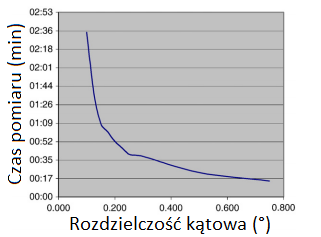
\includegraphics[scale=1]{lasertriangchart.PNG}
  \caption{Czas pomiaru w zależności od dokładności pomiaru \cite{el2008integrating}}   
  \label{fig:lasertriangchart}
\end{figure}